\documentclass[journal,twoside]{IEEEtran}
\usepackage[cmex10]{amsmath}
\usepackage{amssymb}
\usepackage{amsfonts}
\let\proof\relax % needed for amsthm
\let\endproof\relax % needed for amsthm
\usepackage{amsthm}
\usepackage{algpseudocode}
\usepackage{graphicx}
\usepackage{epsfig}
\usepackage{cite}

\graphicspath{{figures/}}
\DeclareGraphicsExtensions{.eps}
\interdisplaylinepenalty=2500

\newtheorem{theorem}{Theorem}
\newtheorem{proposition}{Proposition}
\newtheorem{lemma}{Lemma}
\theoremstyle{definition}
\newtheorem{remark}{Remark}
\newtheorem{assumption}{Assumption}
\newtheorem{definition}{Definition}
\newtheorem{property}{Property}
\newtheorem*{problem}{Problem statement}
\renewcommand\qedsymbol{$\blacksquare$}
\newcommand\T{{\hspace{-0pt}\intercal}}
\newcommand*\diff{\mathop{}\!\mathrm{d}}
\DeclareMathOperator{\sgn}{sgn}

\begin{document}

\title{Design of an Motorised Endoscope Manipulator Interface for Sinus Surgery}

\author{
%David~Navarro-Alarcon,~\IEEEmembership{Member,~IEEE,}~Zerui~Wang,~\IEEEmembership{Student~Member,~IEEE,}~Hiu~Man~Yip,~\IEEEmembership{Student~Member,~IEEE,}
%Yun-hui~Liu,~\IEEEmembership{Fellow,~IEEE,}~Weiyang~Lin,~Jiadong~Shi,~Peng~Li,%
%~Michael~C.~F.~Tong,~Jason~Chan~and~Iris~Leung%
%~ \thanks{This work is supported in part by the Hong Kong RGC under grant 415011 and grant CUHK6/CRF/13G, and in part by the Hong Kong ITF under grant ITS/020/12FP.}%
%\thanks{D. Navarro-Alarcon, Z. Wang, H. M. Yip, Y.-H. Liu and P. Li are with the Department of Mechanical and Automation Engineering, The Chinese University of Hong Kong, Shatin, NT, HKSAR. Corresponding author's phone: +852-39438047; e-mail: navarro-alarcon@cuhk.edu.hk.}%
%\thanks{W. Lin is with the School of Astronautics, Harbin Institute of Technology, Harbin, Heilongjiang, PRC.}%
%\thanks{J. Shi is with the School of Mechatronics Engineering, Beijing Institute of Technology, Beijing, PRC.}%
%\thanks{M. C. F. Tong, J. Chan and I. Leung are with the Department of Otorhinolaryngology, Head and Neck Surgery, Prince of Wales Hospital, Shatin, NT, HKSAR.}%
}

\markboth{IEEE Transactions on , July~2015}%
{Navarro-Alarcon et al. \MakeLowercase{\textit{et al.}}: Design and Sensor-based Control of a Motorised Endoscope Manipulator for Sinus Surgery}
\maketitle


\begin{abstract}
This paper presents the development of an endoscope manipulator interface for the control of active structures for functional endoscopic sinus surgery (FESS).
The motion control system is based on a real-time Linux kernel that processes the commands from the surgeon and controls the manipulator’s active joints.
A user control interface based on an IMU fastened on thesurgeon’s head and a RGB-D sensor(kinect) settled before the user's head is developed is developed; This interface measures the head's posture and position, it provides the desired pan/tilt/zoom motions of the endoscope. 
The developed endoscope manipulator allows the surgeon to conduct ’two-hand’ operations while retaining direct control of the camera.
We present an experimental study to validate the performance of the robotic prototype.

\end{abstract}

\begin{IEEEkeywords}
---Robot manipulators, endoscopic sinus surgery, remote centre of motion, motion control, human-machine interface. 
\end{IEEEkeywords}
\IEEEpeerreviewmaketitle

\section{Introduction}
%~ See Fig. \ref{fig:traditional_surgery}.
%~ 
%~ \cite{Proceedings:Li2013_icia,Proceedings:Lin2015_iros}

\begin{figure}[t]
\centering
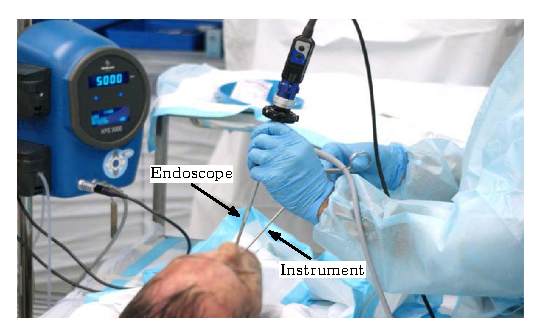
\includegraphics[scale = 1]{fig1}
\caption{In traditional FESS, the surgeon directly manipulates the endoscope.}
\label{fig:traditional_surgery}
\end{figure}
Endoscopes are important imaging devices that are commonly used during minimally invasive surgical operations.
These systems carry a camera and light source that capture in-body images, which are used by the surgeon to conduct
the operation. During traditional functional endoscopic sinus
surgery (FESS), the surgeon uses one hand to manipulate
the endoscope and the other hand to manipulate the surgical
instruments, see Fig. 1. This situation limits the surgeon’s
dexterity during the procedure, where in order to conduct
two-hand operations, an assistant surgeon needs to manipulate the camera (this requires an excellent communication
between both sides). 


\subsection{Related Work}
Many robotic systems have been proposed in the literature
to perform the endoscope manipulation task, see e.g. [1]. A
cable driven surgical endoscope manipulator, with low cost
and easy setup, is presented in [2]; in this work the surgeon
controls the endoscope with voice commands, pedals, a
joystick and head movements.
In [3], a robotic prototype for trans-nasal neurosurgery is
proposed. This endoscope manipulator provides the surgeon
with real-time images, has a 2 rotational joints for pan
and tilt motions, and a 2 translational joints for positioning
the system. In [4], a computer-integrated surgical system
using CAD/CAM models and data from surgical devices is
proposed. The work [5] develops an remote center of motion
(RCM) mechanism and two prototypes of endocavity ultra-
sound probe manipulators. In [6], an endoscope manipulator
with eight motorized joints is proposed for sinus surgery;
this robot is controlled using multiple foot pedals.


\subsection{Contribution}
Our aim in this paper, is to present
a new hand free controlling interface system (head and voice controlled robotic system) that releases the hand-
busy surgeon from the camera manipulation task in a more intuitive way, and enables
him/her to retain direct control of endoscope's position.

\subsection{Organisation} %%%%%%%%%%%%%%%%%%%%%%%%%%%%%%%%%%%%%%%%%%%%%%%%%%%%%%!!!!!
%~ The rest of this paper is organised as follows: Section \ref{sec:design} describes the design of the manipulator; Section \ref{sec:control} derives the control algorithms; Section \ref{sec:experiments} presents the conducted experiments; Section \ref{sec:conclusions} gives final conclusions.
The article is organized as follow. First, in section II we briefly explain the role of every sensors which enables the hand-free
control in a more intuitive way. Then we describe our multisensor framework and algorithm to complete the manipulation
of the controlling signals. In section III we draw a brief conclusion of perfermence about the system and introduce the future work of the development.
\section{Interface and sensor algorithm}\label{sec:design}
In this section, we present and analyse the structure of the proposed endoscope manipulator. 

\subsection{Control system architecture}

The control system is composed of two Linux-based indus-
trial PC, an embedded Galil DMC-1440 control board with
analog outputs, Maxon current amplifiers, electromagnets,
wireless communication modules and an IMU. The Galil
control board decodes the motor’s position and outputs the
analog control signal (calculated by an inner PID algorithm)
to the current amplifiers. One linear joint and two rotary
joints of the active manipulator are controlled in velocity
mode. For safety reasons, the motor of the insertion joint
is controlled in current mode; this joint moves with a
small and constant feed-forward force, which can help to
prevent applying excessive forces to the tissues. A schematic
representation of the control system is shown in Fig. 2.



The control software
is divided into two parts: robot control core and human
machine interface (HMI). The robot control core manages
the hardware resources and is in charge of implementing
the low-level control tasks, such as computing the motor’s
velocity and current commands, enabling and disabling the
algorithms, communicating with the HMI and monitoring the
error events
%~ In traditional endoscopic sinus surgery, the surgeon first inserts the endoscope camera inside the patient's nostril, which serves as a natural pivot point.
%~ With one hand, the surgeon then manipulates the endoscope to observe different regions of interest inside the nasal cavity.
%~ This type of motion consists of two rotations (which control the camera's pan and tilt motions) and one linear translation (which controls the camera's zoom motion).
%~ The camera's roll angle (i.e. the rotation around the optical axis) is typically kept constant throughout the operation, therefore, we intentionally exclude it from our analysis.
%~ See Fig. \ref{fig:rotations} for a conceptual representation of the camera's DOF.

%~ \begin{figure}[t]
%~ \centering
%~ 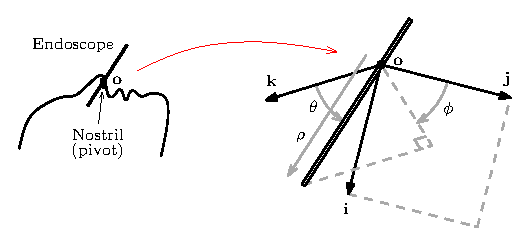
\includegraphics[scale = 1]{fig2}
%~ \caption{Constrained motions of the endoscope, where $\phi$ and $\theta$ represent its orientation, and $\rho$ represents its insertion distance.}
%~ \label{fig:rotations}
%~ \end{figure}

%~ To perform the motions that are necessary to conduct endoscopic sinus surgery, we propose to develop a new robotic system composed of a 5-DOF passive positioning mechanism and a 4-DOF active manipulator. 
%~ The former part allows the surgeon to manually position the system's RCM at the patient's nostril during the set-up stage, the latter part allows the surgeon to actively command the motion of the camera. 
%~ The whole mechanism is placed on a wheeled mobile platform which also houses the motion control system.
%~ See Fig. \ref{fig:conceptual_system} for a conceptual model of the proposed endoscope manipulator.

%~ \begin{figure}[t]
%~ \centering
%~ 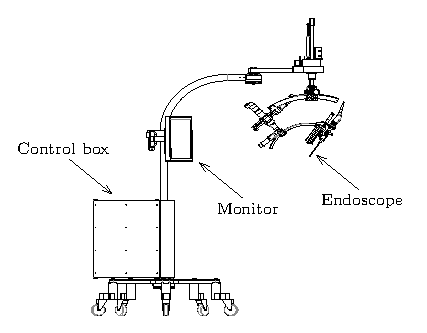
\includegraphics[scale = 1]{fig3}
%~ \caption{Conceptual model of the complete robotic system.}
%~ \label{fig:conceptual_system}
%~ \end{figure}

\subsection{Algorithm of control interface}

 In our system we use an IMU and a RGB-D sensor(kinect) to
control the active manipulator, see Fig. 4. An IMU with an
Arduino micro-controller unit is fastened to the surgeon’s
head to measure the head’s orientation,and the RGB-D camera is settled to measure the head position; the measured feedback
is sent to PC via bluetooth channel and TCP/IP channel respectively. The HMI receives the
feedback data, identifies the head gesture and position from user, and sends
the motion command to the core control application.
The IMU interface measures the pitch and yaw angles
while the kinect measuresthe distant between the user and camera, besides, a microphone is mounted on the user's head to receive speech voice as the highest command to enable and disable the whole system;
 We use these parameters
to implement the following actions: (1) enable/disable the
whole control process, (2)
command the joint’s forward/backward motion.The
interface control logic is described with following set of
rules:

%~ This mechanism has five passive degrees of freedom: four revolute joints and one prismatic joint.
%~ The first four joints $q_1,\ldots,q_4$ form a SCARA-like kinematic structure \cite{Patent:Makino1982}. 
%~ The structure of the fifth joint $q_5$ is a arc gear-rack mechanism that rotates the active manipulator.
%~ See Fig. \ref{fig:passive_mechanism} for a 3D model of this mechanism.
%~ 
%~ The purpose of the SCARA-like structure is to allow the surgeon to manually position the active system in the 3D space during set-up; this structure can also rotate the system along the vertical axis.
%~ The purpose of the arc joint $q_5$ is to allow the surgeon to set with a manual handle the desired `home' orientation for the motorised tilting angle of the camera (to be described in the next section)
%~ 
%~ The vertical joint $q_4$ provides linear up-and-down motions to the system. 
%~ This mechanism is gravity-balanced so that it can be easily positioned by the surgeon during set-up.
%~ To implement this behaviour, we use the following components: an air-spring, a spline axis, a damper, and an electromagnetic (EM) lock.
%~ The air-spring can support a load of nearly 80N; we incorporate a damper to stabilise the force of this component.
%~ 
%~ Once the endoscope camera has the desired position and orientation inside the patient's nasal cavity, the passive positioning mechanism can be fixed with a series of EM locks that are embedded into the joints $q_2$, $q_3$, and $q_4$.
%~ These breaks are activated/deactivated with a simple on/off switch.

%~ \begin{figure}[t]
%~ \centering
%~ 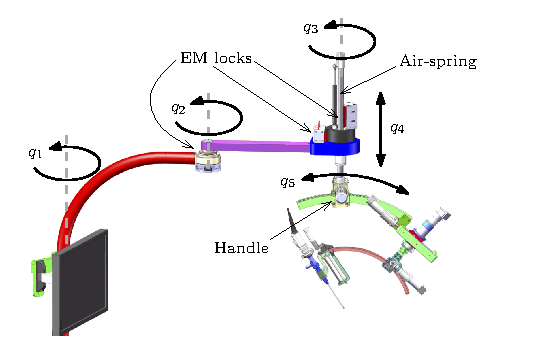
\includegraphics[scale = 1]{fig4}
%~ \caption{The passive positioning mechanism.}
%~ \label{fig:passive_mechanism}
%~ \end{figure}

%~ \subsection{Active Endoscope Manipulator}
%~ The structure of the active manipulator is depicted in Fig. A.
%~ This system has four motorised degrees of freedom, two prismatic joints and two revolute joints, all driven by DC motors.
%~ The prismatic joints $q_6$ and $q_9$ have a ball-screw structure; the joint $q_7$ directly rotates an arc gear-rack mechanism that is driven by joint $q_8$.
%~ 
%~ The purpose of the linear joint $q_6$ is to translate the RCM point into its desired location (i.e. inside the patient's nostril).
%~ For that, the active manipulation most be first manually adjusted with the passive mechanism such that the axis of $q_6$ is parallel to the sinus cavity.
%~ Note that this motorised joint is not used very often during the operation; we only use it during set-up or whenever there is the to readjust the RCM point (e.g. when changing the patient's posture).
%~ 
%~ The purpose of the last three joints $q_7$, $q_8$ and $q_9$ is to control the pan, tilt, and zoom motion of the endoscope camera, respectively. 
%~ The axes of motion of the rotational joints $q_7$ and $q_8$ are designed such that they are always orthogonal, and the intersection of its axes determines the RCM point of the manipulator.
%~ To prevent injures resulting from large motions, the fixed RCM point must be set at the entry of the patient's nostril.

\begin{figure}[t]
\centering
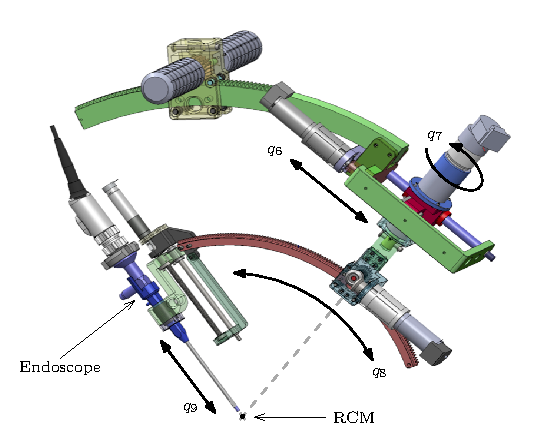
\includegraphics[scale = 1]{fig5}
\caption{The active endoscope manipulator.}
\label{fig:active_manipulator}
\end{figure}

%~ \subsection{Kinematics}


%The last three active joints of the system are designed such that its displacements directly control the pan, tilt and zooming motion of the camera.With these DOF, we can represent the constrained configuration of the endoscope with spherical coordinates, i.e. joints $q_7=\phi$, $q_8=\theta$ and $q_9=\rho$ (see Fig. \ref{fig:rotations}).

%~ From Fig. \ref{fig:rotations}, we can see that the constrained 3-DOF configuration of the endoscope can be locally represented with spherical coordinates.
%~ The specific design of the active endoscope manipulator allows us to control this configuration directly with the last three joints.
%~ To this end, we must first define the `home' (i.e. zero) configuration by rotating joint $q_8$ such that the axes $q_6$ and $q_9$ are parallel.
%~ With this reference configuration, the joint $q_7=\phi$ represents the angle measured over the plane $(\mathbf i,\mathbf j)$, the joint $q_8=\theta$ represents the angle between the endoscope and the axis $\mathbf k$, and the joint $q_9=\rho$ represents the insertion distance.
%~ 
%~ We can compute the Cartesian position vector $\mathbf p\in\mathbb R^3$ of the endoscope's tip with the following expression:
%~ \begin{equation}
				%~ \mathbf p = \rho
				%~ \begin{bmatrix}
								%~ \sin(\theta) \cos(\phi) & 
								%~ \sin(\theta) \sin(\phi) &
								%~ \cos(\theta)
				%~ \end{bmatrix}^\T.
%~ \end{equation}
%~ The coordinates of the vector $\mathbf p$ are defined with respect to the RCM point $\mathbf o$.


%~ \section{Controller Design}\label{sec:control}
%~ In this section, we describe the developed control system and propose hand-free methods to control the position of the manipulator.
%~ 
%~ \subsection{Motion Control System}
%~ The motion control system that we developed for this robot is composed of a low-level industrial motion controller, and a high-level PC-based controller.
%~ As the low-level controller, we use a Galil DMC-1440 motion servo-controller; this embedded board decodes the motors' positions and outputs the current control signals (calculated by an inner PID algorithm) that drive the DC motors.
%~ As the high-level controller, we use an industrial PC (i5-3550S CPU) running a Linux-based operative system; this PC processes all external sensor feedback and computes the motion control algorithms.
%~ The communication between the low-level and high-level modules is done via high-speed Ethernet.
%~ All the motorised joints of the manipulator are controlled in velocity-mode, with a servo-loop of $10$ milliseconds.
%~ See Fig. \ref{fig:motion_controller} for a schematic representation.
%~ 
%~ To guarantee the absolute safety during the surgical procedure, the control system must operate with a strict (i.e. deterministic) real-time behaviour.
%~ We provided this valuable feature to our high-level controller by installing a Linux kernel with a customised real-time patch. 
%~ For that, we use the Xenomai real-time development framework, see \cite{Misc:Gerum2004} for details.
%~ 
%~ To develop the hand-free user interface for the motorised manipulator, we integrate different sensors into our system.
%~ We use an inertial measurement unit (IMU) to measure the orientation/posture of the user's body; the measured angles from this device are processed with a microcontroller board (Arduino Uno) and are wirelessly transmitted to the PC with Bluetooth device at 57600 bps.
%~ To process in real-time the captured images from the endoscope camera, we use a digital TV-card (Hauppauge) with USB interface.
%~ The design of these control interfaces is described in the following sections.
%~ 
\begin{figure}[t]
\centering
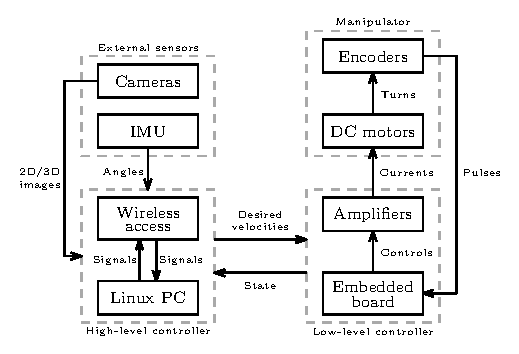
\includegraphics[scale = 1]{fig6}
\caption{Schematic representation of the motion control system.}
\label{fig:motion_controller}
\end{figure}
%~ 
%~ \subsection{Foot-controlled Interface}
%~ % general idea / problem
%~ The purpose of our robotic manipulator is to enable the surgeon to conduct two-hand operations (i.e. to simultaneously manipulate two instruments) while retaining direct control over the endoscope camera.
%~ To achieve this objective, we developed an IMU-based interface that uses foot gestures to control the camera motions.
%~ This device is attached to the user's foot, as shown in Fig. \ref{fig:imu_foot}.
%~ 
%~ \begin{figure}[t]
%~ \centering
%~ 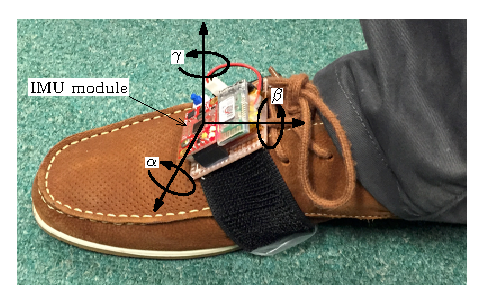
\includegraphics[scale = 1]{fig7}
%~ \caption{The foot-controlled interface with its orientation angles.}
%~ \label{fig:imu_foot}
%~ \end{figure}
%~ 
%~ % what and how you did it / meaning
%~ With the IMU device, we measure the orientation angles $\alpha,\beta,\gamma\in\mathbb R$ of the user's foot in real-time; we use these feedback angles to control the last three motorised joints (i.e. the pan, tilt, and zoom joints) of the manipulator.
%~ Note that the control of the endoscope's position with a foot gesture is a difficult task because the motion of the foot is not as dexterous as the motion of a hand.
%~ For this reason, with our proposed foot interface we only control one joint of manipulator at the time and with a constant speed command.
%~ The developed interface has implemented the following actions: (1) enable/disable the control interface, (2) select the active joint, and (3) command the forward/backward motion.
%~ Fig. \ref{fig:foot_enable} and Fig. \ref{fig:foot_gestures} graphically depict the implemented foot gestures. 
%~ 
%~ % details / algorithm
%~ The control logic of this interface is detailed in the following pseudocode:
%~ \begin{algorithmic}[1]
				%~ \Loop \Comment{Main loop of the foot-controlled interface}
					%~ %\If{$\alpha<10^\circ \rightarrow \alpha> 60^\circ \rightarrow \alpha<10^\circ \rightarrow \alpha> 60^\circ$}
					%~ \If{$Voiceinput\ \ ==\ \ 'activate'$}
						%~ \State Enable interface 
					%~ \EndIf
					%~ 
					%~ \If{$Voiceinput\ \ ==\ \ 'stop'$}
						%~ \State Disable interface 
					%~ \EndIf
					%~ 
					%~ \If {Interface enabled}
						%~ \If {$\alpha<10^\circ$ and $(\beta<-15^\circ \rightarrow \beta>15^\circ)$}
							%~ \State Change active joint
						%~ \ElsIf {$10^\circ \le \alpha\le60^\circ$ and $|\gamma|>15^\circ$}
							%~ \State Move active joint in the direction of $\sgn(\gamma)$
						%~ \ElsIf {No command for 10 seconds} 
							%~ \State Disable interface
						%~ \EndIf
					%~ \EndIf 
				%~ \EndLoop
%~ \end{algorithmic}
%~ 


%~ (explain with words this algorithm)
%~ 
%~ In this algorithm we use the symbol $A \rightarrow B$ to represent the transition from state $A$ to state $B$. 
%~ Note that the threshold parameters (e.g. $10^\circ$) can be calibrated during set-up depending on the user requirements.
%~ The ``change active joint'' command incrementally shift among the last three motorised joints, i.e. from $q_7\rightarrow q_8\rightarrow q_9\rightarrow q_7\rightarrow\cdots$ and so on.
%~ To facilitate the operation of the interface, the commands are automatically verbalised by the system as follows: ``enabled'', ``disabled'', ``pan'', ``tilt'', and ``zoom''.
%~ 
%~ \begin{figure}[t]
%~ \centering
%~ 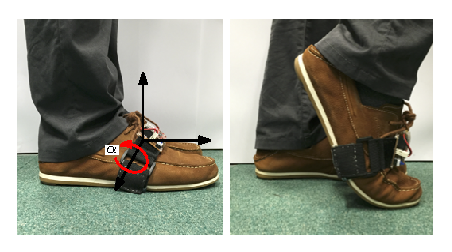
\includegraphics[scale = 1]{fig8}
%~ \caption{The gesture to enable/disable the foot-controlled interface.}
%~ \label{fig:foot_enable}
%~ \end{figure}
%~ 
%~ \begin{figure}
%~ \centering
%~ 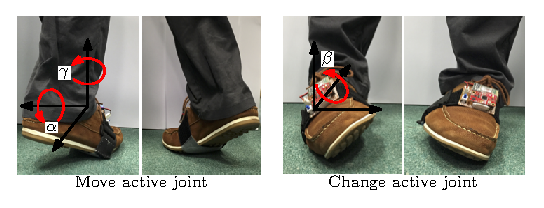
\includegraphics[scale = 1]{fig9}
%~ \caption{The foot gestures to (left) command forward/backward motion to the joint and (right) change the current active joint.}
%~ \label{fig:foot_gestures}
%~ \end{figure}
%~ 
%~ \subsection{Head-controlled Interface}
%~ % general idea / problem
%~ In this section we describe the design of an interface that uses head motions to control the endoscope camera.
%~ As with the previous approach, we use an IMU module to measure the orientation of the head. 
%~ We additionally integrate an RGB-D sensor (Kinect) to measure 3D displacements of the head, and a wireless microphone to allow the user to use voice commands.
%~ The developed head-controlled interface is depicted in Fig. \ref{fig:imu_head}.
%~ 
\begin{figure}[t]
\centering
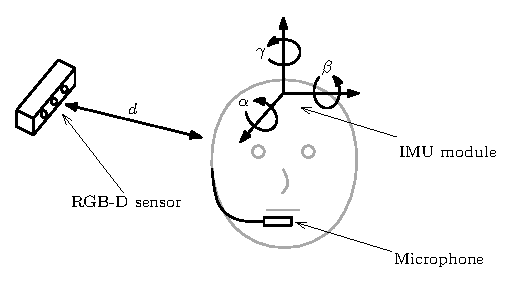
\includegraphics[scale = 1]{fig10}
\caption{The head-controlled interface with orientation angles, and microphone.}
\label{fig:imu_head}
\end{figure}
%~ 
%~ % what and how you did it / meaning
%~ By using head motions, we can implement a more natural relation between the gestures of the user and the motion of the camera.
%~ In our approach, we use the ``up/down'' angle $\beta$ to control the camera's tilting (i.e. vertical) motion, and the ``left-right'' angle $\gamma$ to control the camera's pan (i.e. horizontal) motion.
%~ In our set-up, the RGB-D sensor is placed on top of the surgeon's monitor, therefore, we can measure the scalar distance $d$ between the head and the monitor in real-time; we use this relative distance (or proximity) to control the zooming motions of the camera.
%~ To enable/disable the interface, two simple voice commands are implemented: ``enable control'' and ``stop control''. 
%~ We use speech recognition algorithms (CMU Pocketsphinx libraries) to automatically detect these commands.
%~ For safety reasons, only one joint of the robot can be controlled at the time.
%~ Fig. \ref{fig:head_gestures} depicts the implemented head gestures.
%~ 
%~ % details / algorithm
%~ The control logic of the interface is detailed in the following pseudocode:



\begin{algorithmic}[1]
				\Loop \Comment{Main loop of the head-controlled interface}
					\If{``enable/stop control'' command is detected}
						\State Enable/disable interface 
					\EndIf
					\If {Interface enabled}
						\If {$|\gamma|>30^\circ$}
							\State Move joint $q_7$ in the direction of $\sgn(\gamma)$
						\ElsIf {$|\beta|>30^\circ$}
							\State Move joint $q_8$ in the direction of $\sgn(\beta)$
						\ElsIf {$|d - d_0|>10$cm}
							\State Move joint $q_9$ in the direction of $\sgn(d - d_0)$
						\ElsIf {No command for 10 seconds} 
							\State Disable interface
						\EndIf
					\EndIf 
				\EndLoop
\end{algorithmic}
%~ 
In this algorithm we use the symbol $\gamma$ to represent the
panning directionof user's head. Note that the threshold pa-
rameters (e.g. 10◦ ) can be calibrated during set-up depending
on the user requirements. Different joints are controlled by $\gamma$, $\beta$ and $d$ each standing for panning tilting and zooming of the endoscope respectively. To facilitate the
operation of the interface, the commands are automatically
verbalised by the system as follows: “enabled”, “disabled”,
“pan”, “tilt”, and “zoom”.
%~ % explain algorithm
%~ The purpose of this method is to provide the surgeon with an intuitive way to control the camera: e.g. by rotating the head to the left the camera then rotates to the left, or by approaching to the monitor the camera zooms-in.
%~ Similarly to the previous interface, the threshold parameters can be calibrated during the system's set-up depending on the user's requirements.
%~ 
%~ \begin{figure}[t]
%~ \centering
%~ 
\includegraphics[scale = 1]{fig11}
%~ \caption{The head gestures to command the motion of the endoscope manipulator.}
%~ \label{fig:head_gestures}
%~ \end{figure}
%~ 
%~ 
%~ \subsection{Automatic Image-based Instrument Tracking}
%~ % general idea / problem
%~ In this section we present an uncalibrated controller to automatically track the instrument manipulated by the surgeon.
%~ To achieve this objective, we integrate into the control system the image feedback captured by the endoscope camera.
%~ The purpose of this approach is to automatically move the instrument to the centre of the captured scene, which allows the surgeon to observe specific areas inside the nasal cavity. 
%~ Similarly to the head-controlled interface, we also use a microphone to enable this auto-track control modality.
%~ 
%~ % what and how you did it / meaning
%~ The design of the controller is based on captured images of the surgical instrument, see Fig. \ref{fig:image-based_tracking} for a conceptual representation of the set-up. 
%~ Let us define the \emph{imaged} tip of the instrument by $\mathbf m\in\mathbb R^2$.
%~ The desired image position of the tip is defined by $\mathbf m_d\in\mathbb R^2$, which in our application represents the centre coordinates of the capture image.
%~ With this controller, we only consider the motion of the pan and tilt joints, i.e. joints $q_7$ and $q_8$.
%~ For ease of presentation, we define the input velocity vector $\dot{\mathbf q}\in\mathbb R^2$ as follows:
%~ \begin{equation}
				%~ \dot{\mathbf q}=
				%~ \begin{bmatrix}
								%~ \dot{q}_7 & \dot{q}_8
				%~ \end{bmatrix}^\T
%~ \end{equation}
%~ 
%~ From standard visual servoing [], we know that there exists a differential kinematic relation between the input motion $\dot{\mathbf q}$ of the moving camera and the measured optical flow $\dot{\mathbf m}$ of the image point.
%~ We model this differential relation as follows:
%~ \begin{equation}
				%~ \dot{\mathbf m} = \mathbf J \dot{\mathbf q}
%~ \end{equation}
%~ where the square matrix $\mathbf J\in\mathbb R^{2\times 2}$ denotes the image Jacobian matrix, which depends on the camera's calibration parameters and the 3D Cartesian position of the instrument.
%~ Note that since the instrument is manipulated by the surgeon, its 3D position vector is not known to us and is difficult to estimate using 2D images from a monocular camera.
%~ Therefore, the matrix $\mathbf J$ cannot be analytically computed. 
%~ To cope with this issue, in this work we propose to compute an adaptive estimation, here denoted by $\widehat{\mathbf J}\in\mathbb R^{2\times 2}$, of the unknown Jacobian matrix.
%~ 
%~ \begin{figure}[t]
%~ \centering
%~ 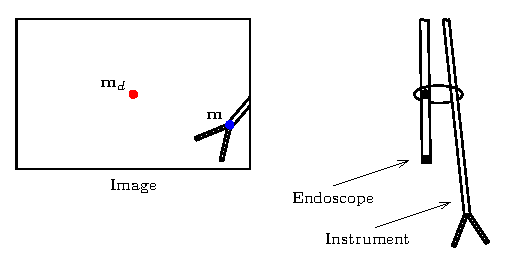
\includegraphics[scale = 1]{fig12}
%~ \caption{Conceptual representation of the image-based instrument tracking control.}
%~ \label{fig:image-based_tracking}
%~ \end{figure}
%~ 
%~ Consider the following definition of the scalar functional 
%~ \begin{equation}
				%~ H = \frac{1}{2} \left\| \widehat{\mathbf J}\dot{\mathbf q} - \dot{\mathbf m} \right\|^2
%~ \end{equation}
%~ which quantifies the accuracy of the estimated matrix $\widehat{\mathbf J}$.
%~ In our method, we vary the elements $\widehat{J}_{ij}\in\mathbb R$ of this matrix with the gradient descent rule
%~ \begin{equation}
				%~ \frac{\diff}{\diff t} \widehat{J}_{ij} = - \lambda \frac{\partial H}{\partial\widehat{J}_{ij}}
%~ \end{equation}
%~ where the scalar $\lambda\in\mathbb R$ represents a positive tuning gain; Appendix \ref{apx:stability} presents the stability analysis of this adaptive estimator.
%~ With our uncalibrated adaptive method, we compute the velocity control input as 
%~ \begin{equation}
				%~ \dot{\mathbf q} = - k \widehat{\mathbf J}^{-1}\Delta\mathbf m
%~ \end{equation}
%~ where $k\in\mathbb R$ denotes a positive (proportional-like) feedback gain, and $\Delta\mathbf m=\mathbf m-\mathbf m_d\in\mathbb R^2$ denotes the image error.
%~ 
%~ % details / algorithm
%~ The following pseudocode details the implementation of our method
%~ 
%~ % explain algorithm
%~ 
%~ 
%~ 
%~ 
%~ 
%~ 
%~ \section{Experiments}\label{sec:experiments}
%~ In this section, we present the developed robotic prototype and then conduct several experiments to evaluate its performance.
%~ 
%~ \subsection{Developed Prototype}
%~ 
%~ \subsection{Control with Foot Gestures}
%~ 
%~ \subsection{Control with Head Motions}
%~ 
%~ \subsection{Image-based Instrument Tracking}
%~ 
%~ \subsection{Ex-vivo Cadaver Test}

\section{Conclusions}\label{sec:conclusions}

In this paper, we developed a new surgical endoscope
manipulator to assist the surgeon during a FESS. The system
is composed of a 5-DoF passive positioning arm, and a
4-DoF active robotic manipulator. To control its motion,
we proposed an IMU-based human-robot interface which is
attached to the surgeon foot; the ex-vivo experiments showed
that this interface is intuitive and easy to use.
As future work, we would like to incorporate automatic
control mode into the system, e.g. the use of image-based
method to automatically position the endoscopic camera
inside the nasal cavity. To improve the safety of the system,
we would like to integrate the feedback of a force/moment
sensor into our control methods.


%~ \section*{Acknowledgements}
%~ We would like to express our gratitude to Dr. Zhifeng Wang for his early mechanical design of the system.

%~ \appendices
%~ \section{Stability Analysis of the Jacobian Estimator}\label{apx:stability}




\ifCLASSOPTIONcaptionsoff
  \newpage
\fi

\bibliography{bib}
\bibliographystyle{IEEEtran}


\end{document}


